\documentclass{article}

\title{CPS 8316 Assignment 3}
\date{April 2022}
\author{Kody Manastyrski}

\usepackage{amsmath}
\usepackage{amsfonts}
\usepackage{mathtools}

\usepackage{rotating}
\usepackage{graphicx}
\usepackage{subcaption}

\begin{document}
\maketitle

\section{Question 1}

To calculate a voronoi diagram for disjoint line segments, we may simply modify
any existing algorithm as follows:
Calculate the voronoi cells for the endpoints of the line segments.
Join the cells for 2 segments by extending a rectangle of width $2\epsilon$ between them, where
epsilon is a constant < 1.  
Next we check if the rectangle intersects any other cells.
If it does, then we find the points where intersection begins/ends.
From these points we then find the point on the line segments that defines the two cells, and
calculate the voronoi cells for those spots. 
If the rectangle does not intersect a cell, double epsilon.
If on the other hand a cell intersects the line segment, place a point at the intersection, and calculate the
voronoi cell between the point defining the cell, and the intersection point. 

\begin{figure}[h!]
	\centering
	
	\begin{subfigure}{0.3\linewidth}
		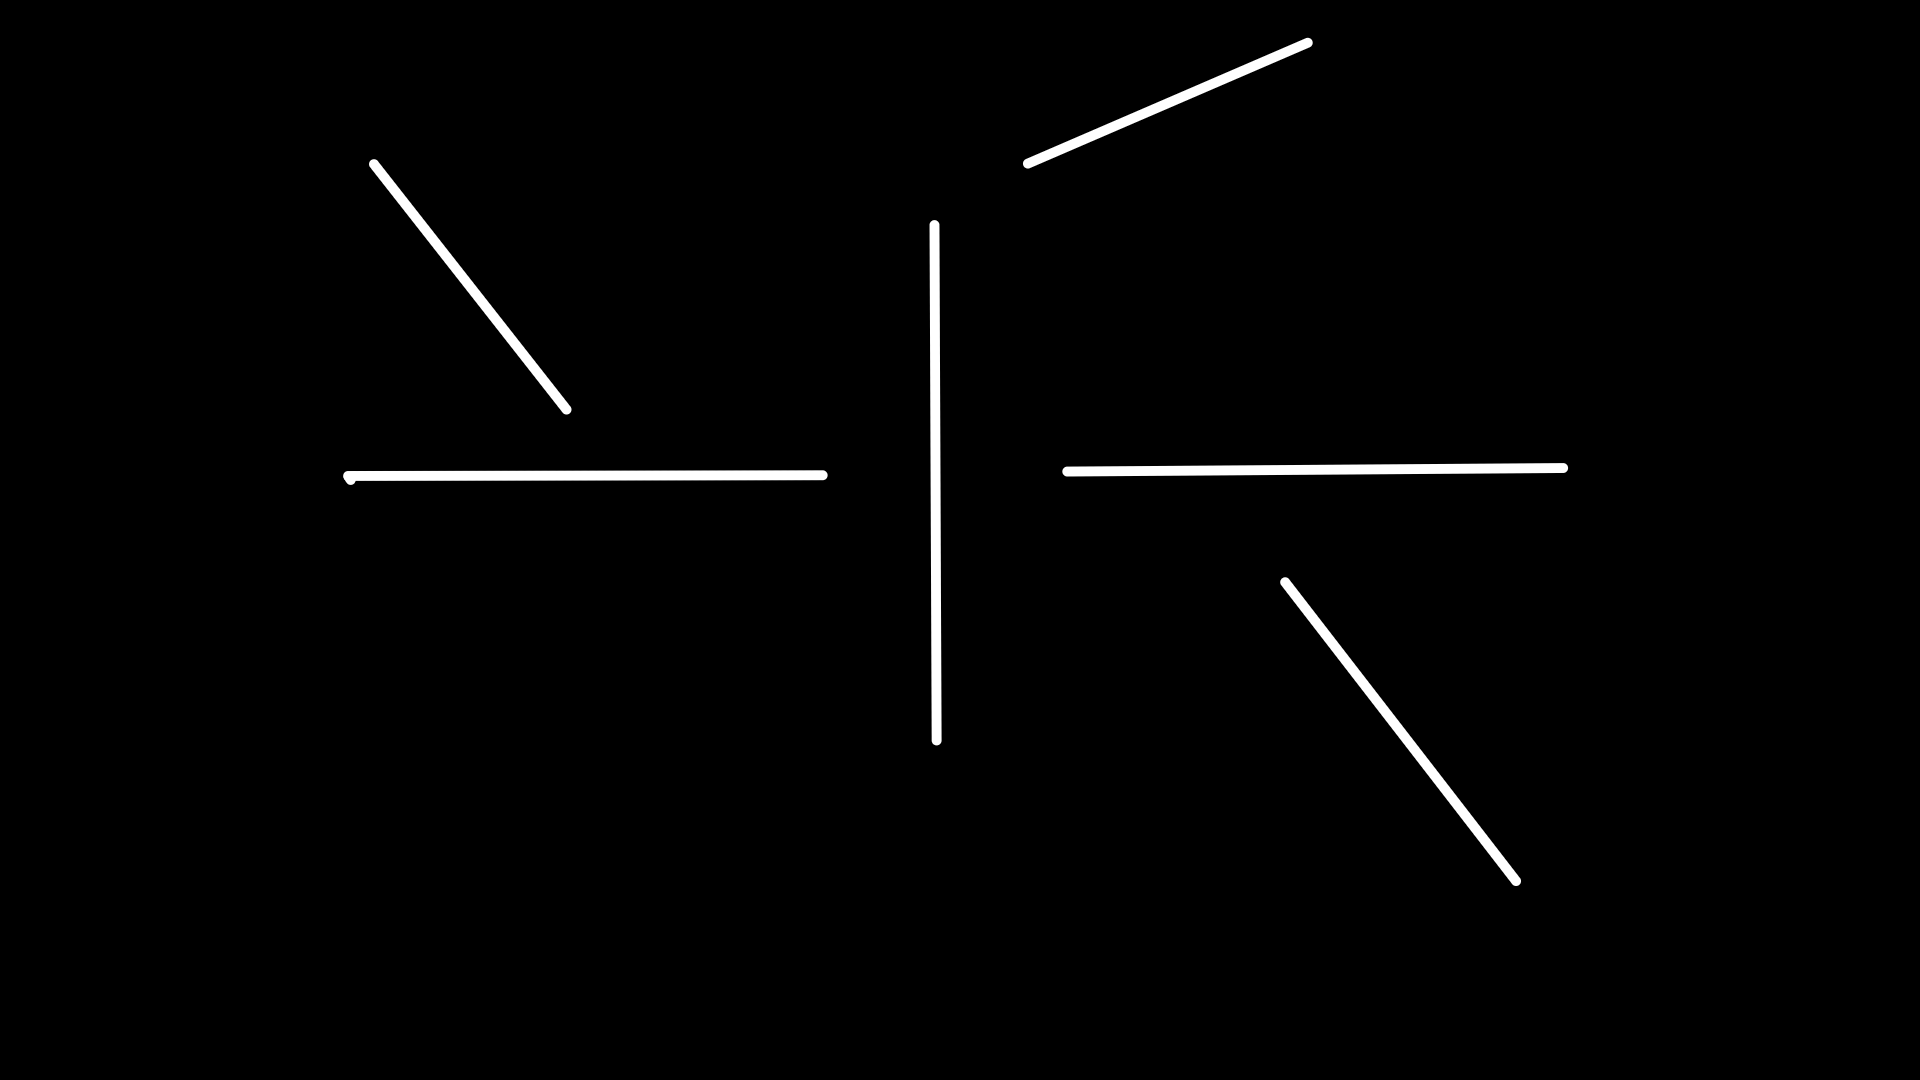
\includegraphics[width=\linewidth]{Step1.png}
		\caption{Initial Conditions, an arrangement of line segments}
		\label{fig:Step1}
	\end{subfigure}%
	\hfill
	\begin{subfigure}{0.3\linewidth}
		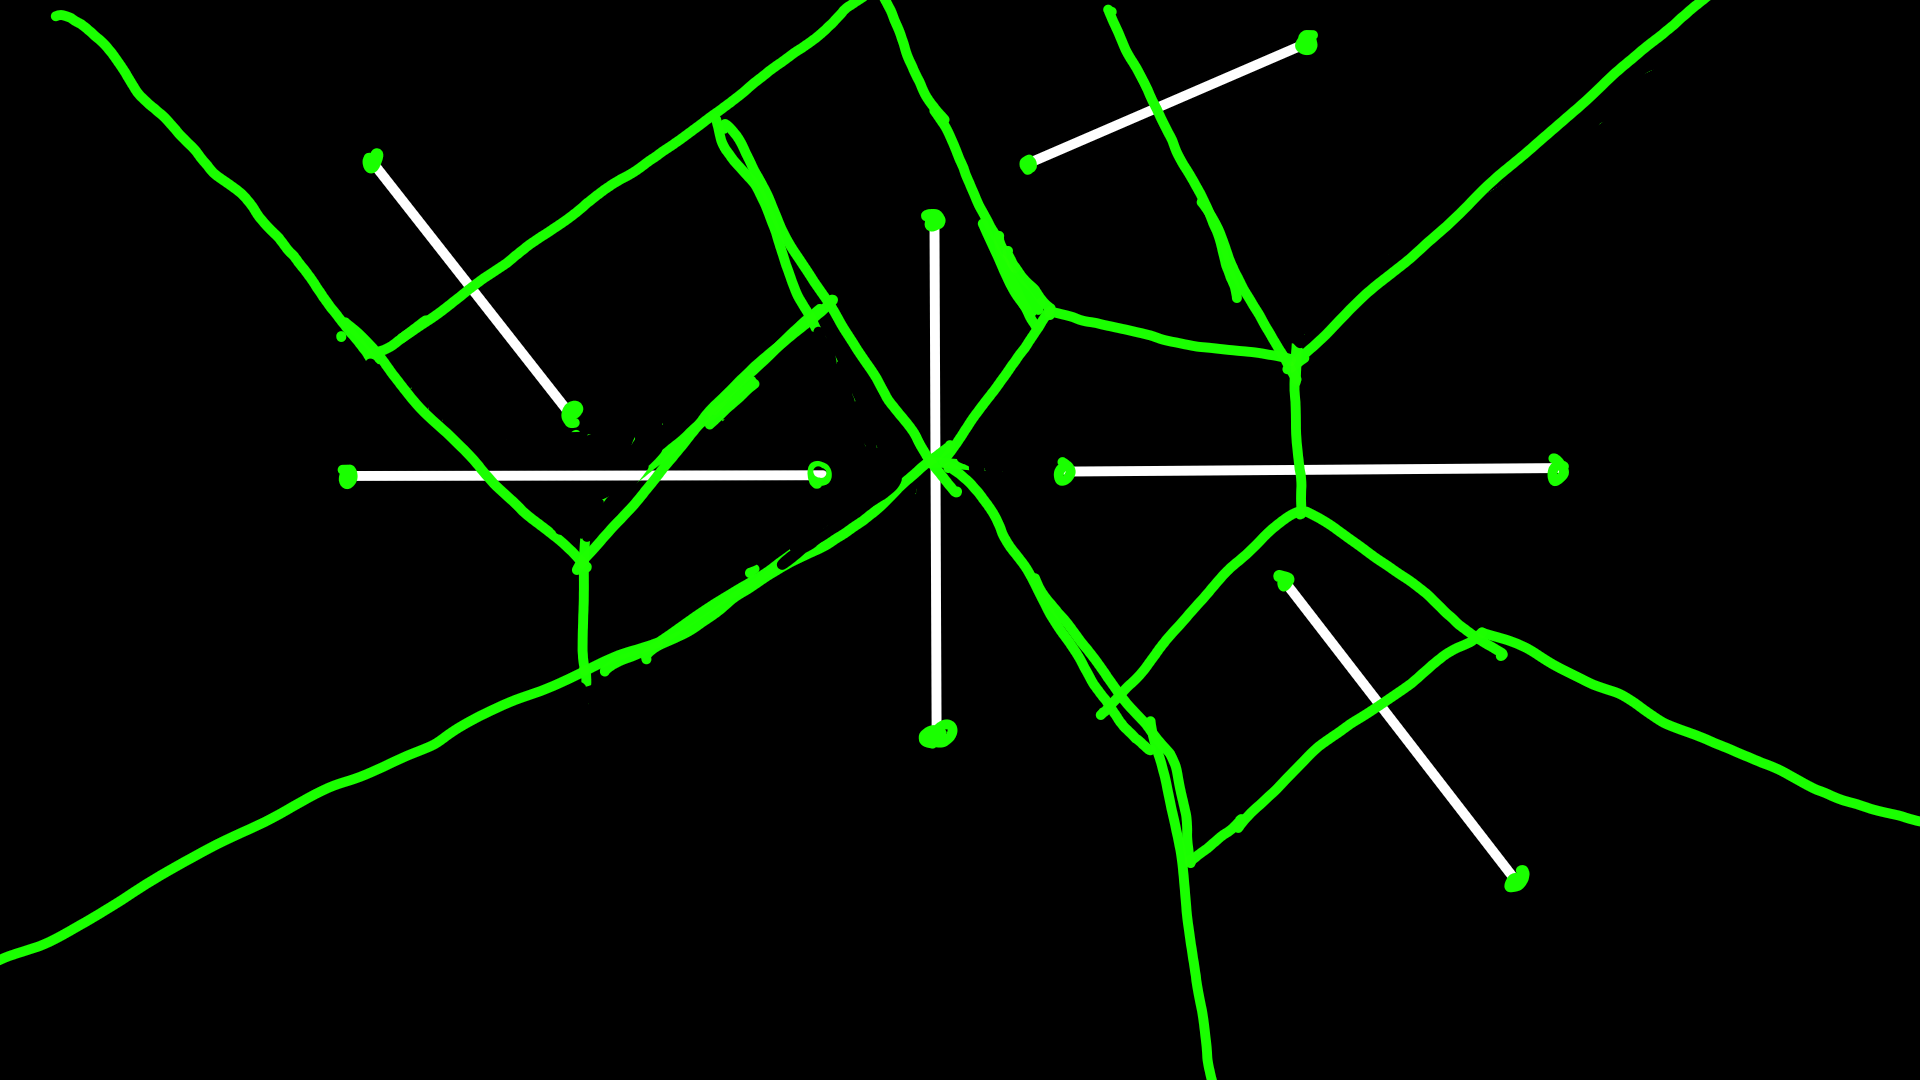
\includegraphics[width=\linewidth]{Step2.png}
		\caption{Calculate voronoi diagrams for segment endpoints}
		\label{fig:Step2}
	\end{subfigure}%
	\hfill
	\begin{subfigure}{0.3\linewidth}
		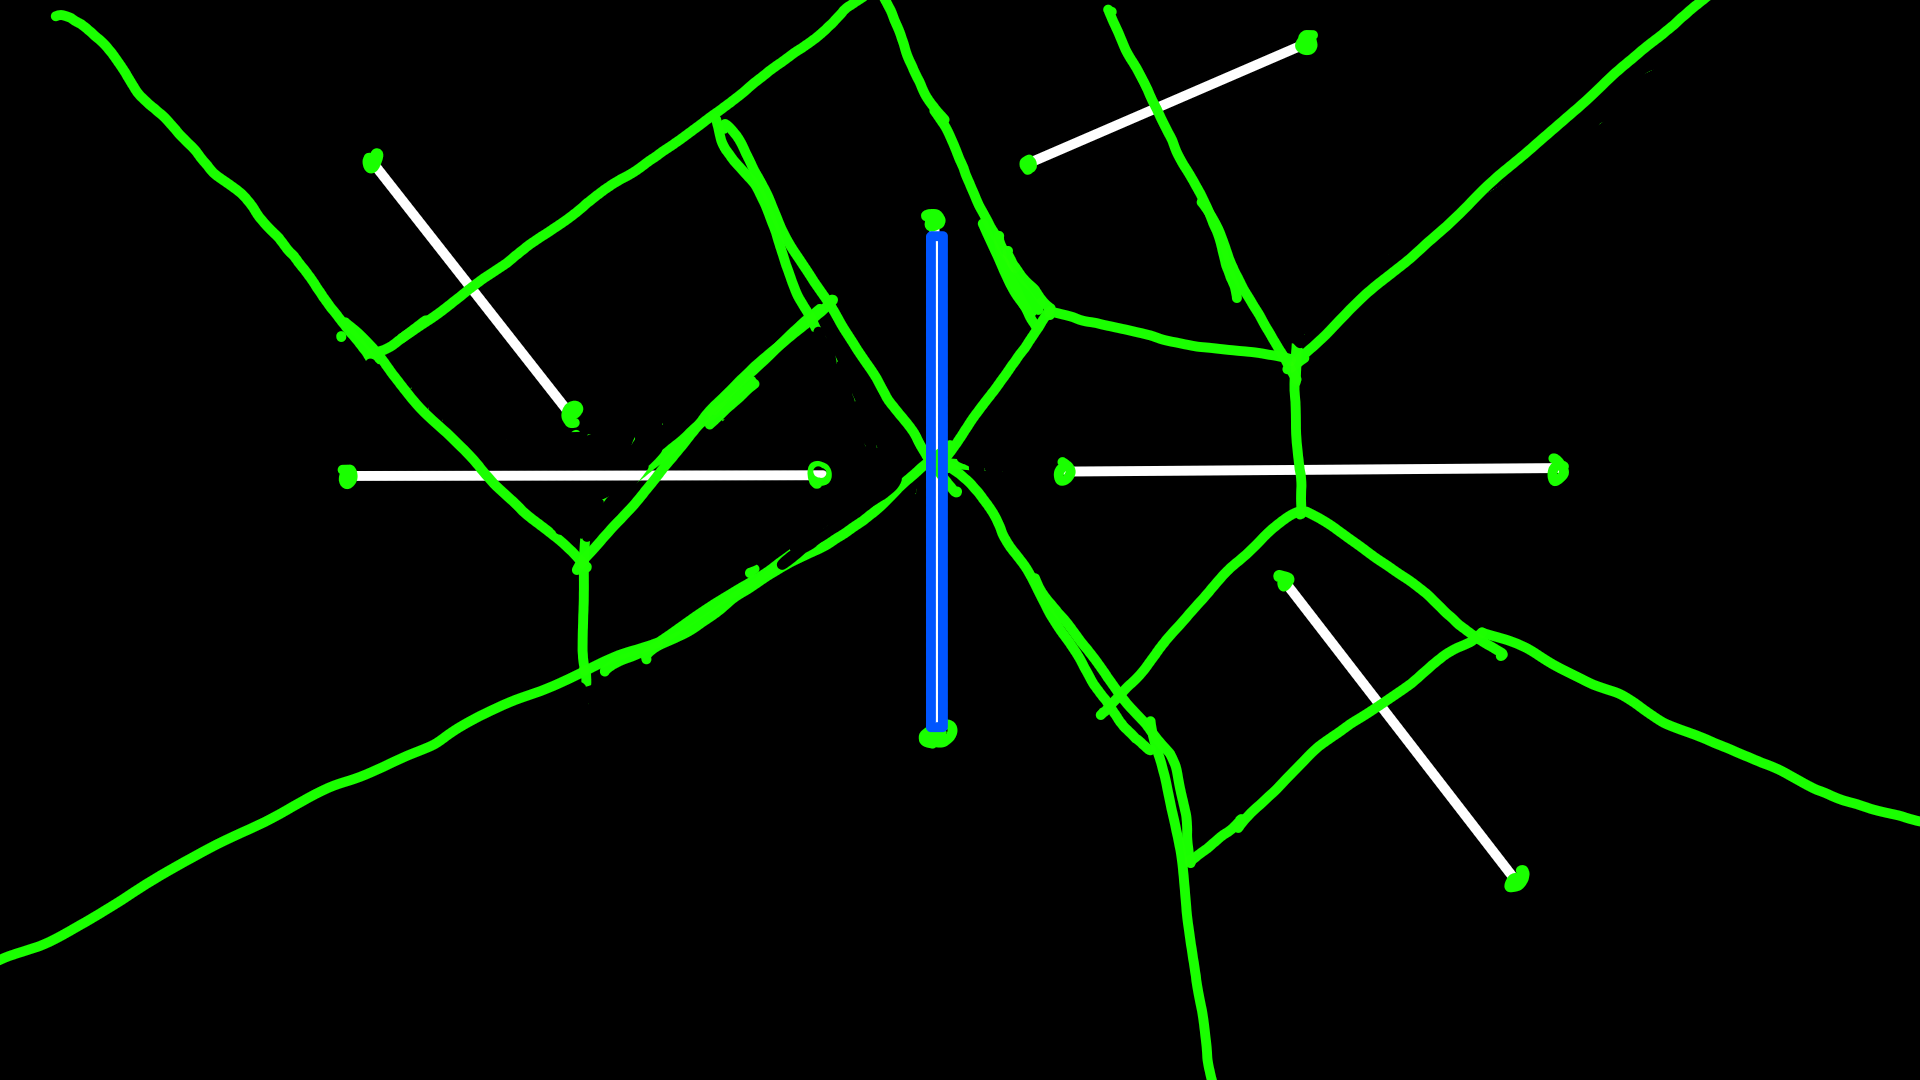
\includegraphics[width=\linewidth]{Step3.png}
		\caption{Extend rectangle between two endpoints sharing a line segment}
		\label{fig:Step3}
	\end{subfigure}
\end{figure}

\begin{figure}[h!]
	\centering

	\begin{subfigure}{0.3\linewidth}
		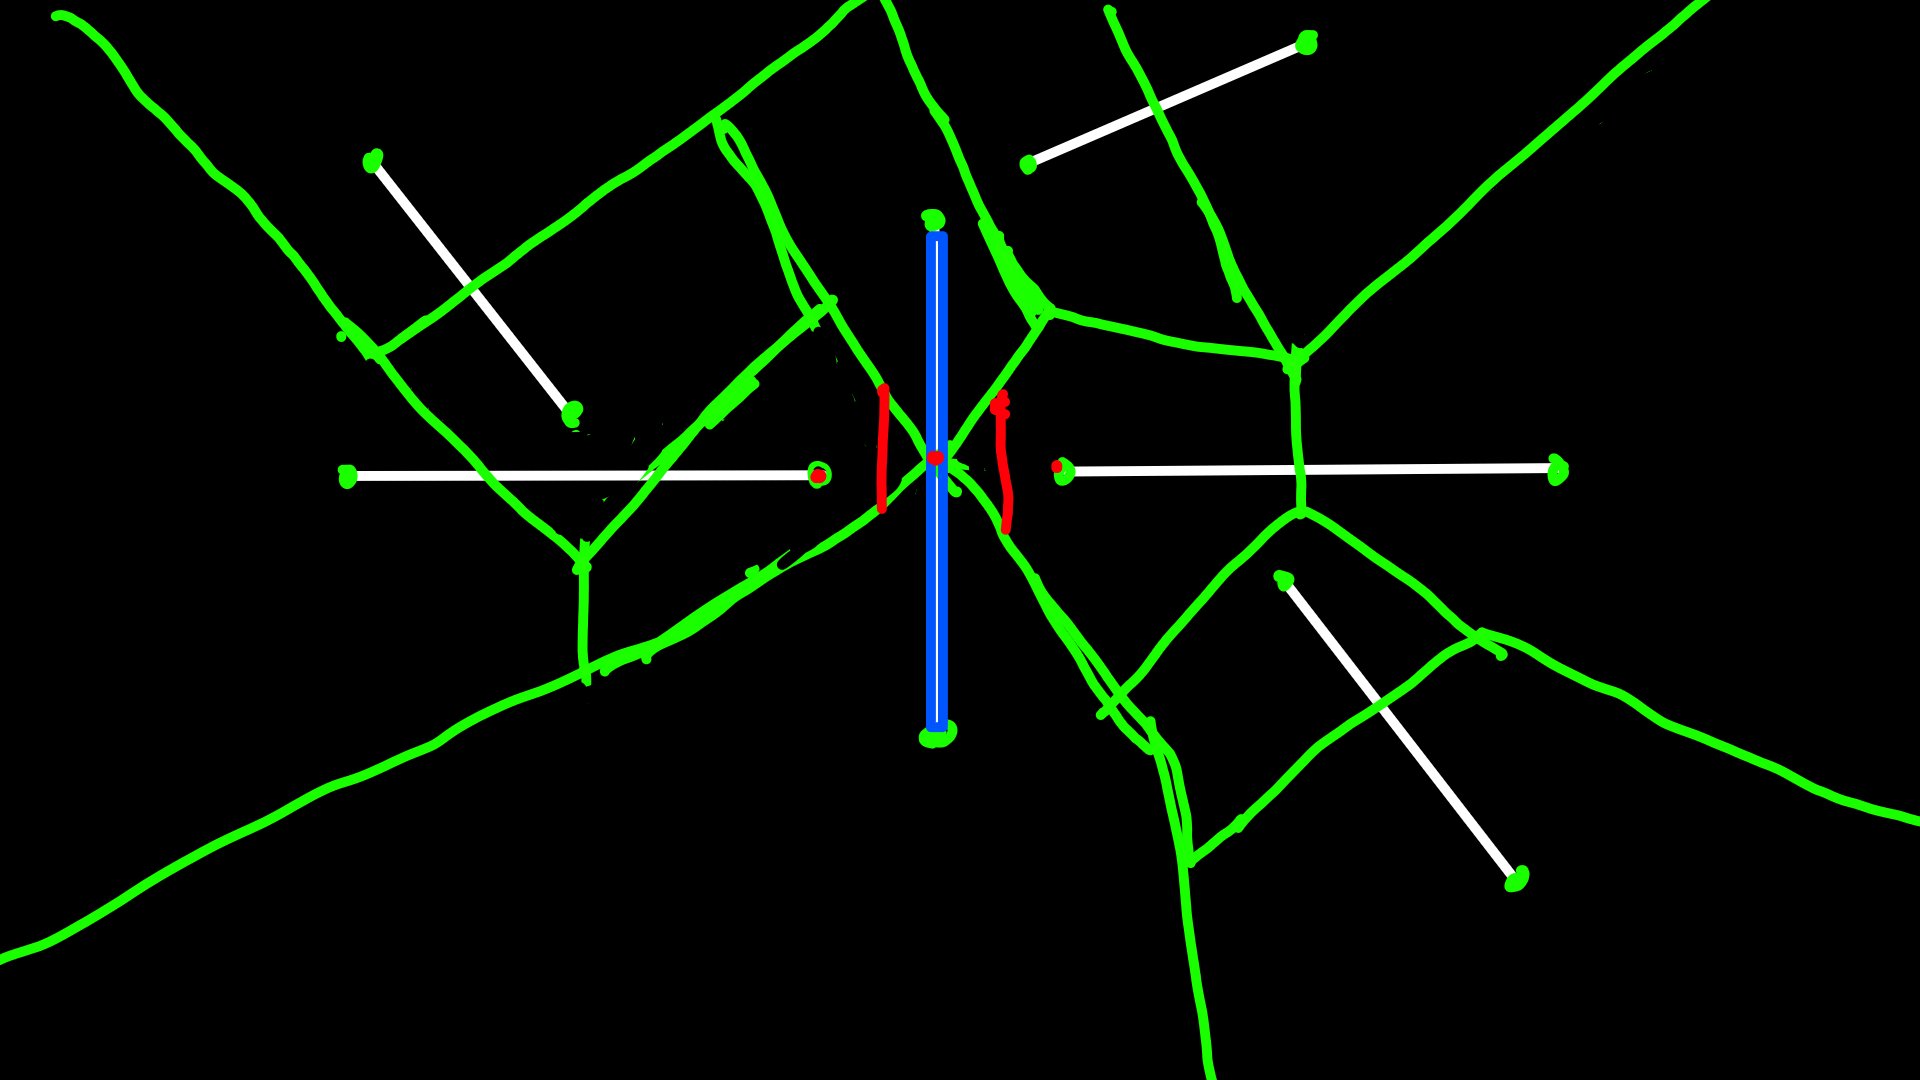
\includegraphics[width=\linewidth]{Step4.png}
		\caption{Widen rect., find closest points between conflicting segments, calculate the voronoi between points}
		\label{fig:Step4}
	\end{subfigure}%
	\hfill
	\begin{subfigure}{0.3\linewidth}
		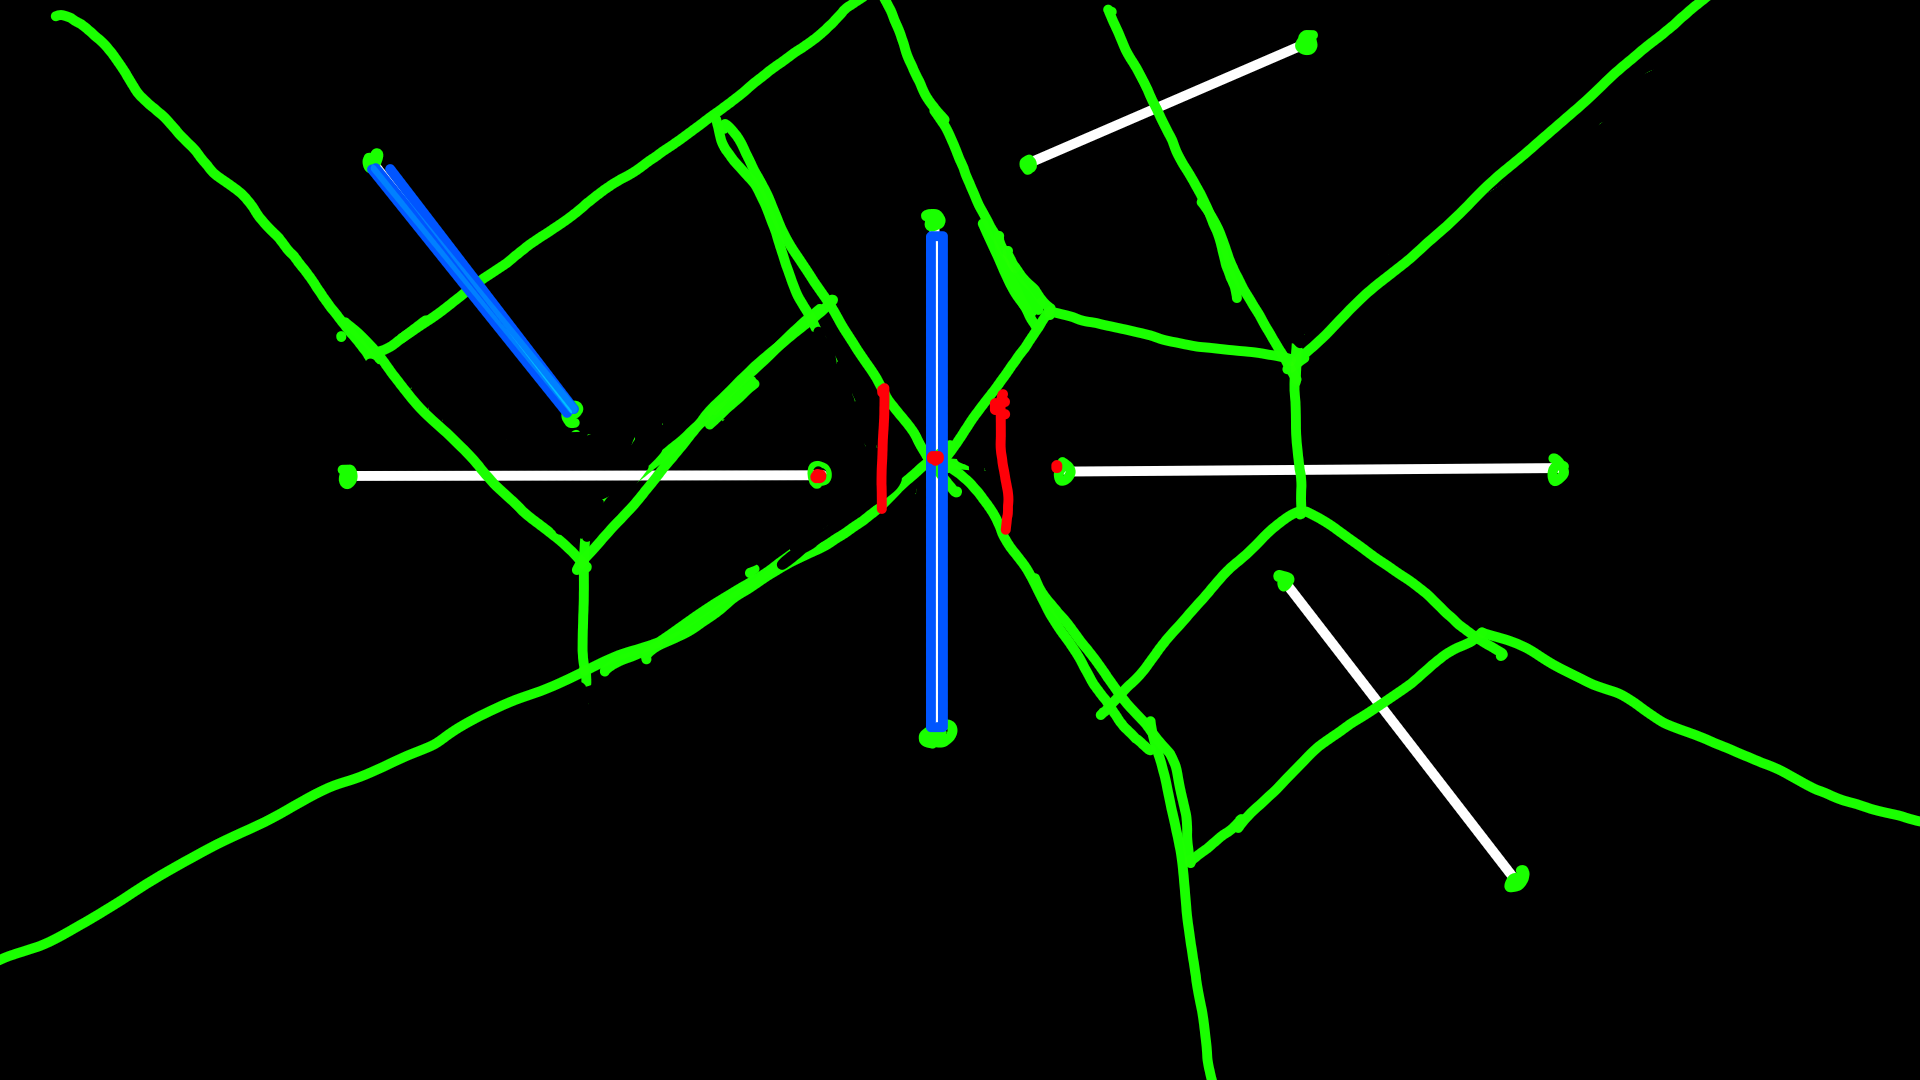
\includegraphics[width=\linewidth]{Step5.png}
		\caption{Extend rectangle for another line segment to join their respective cells and look for conflicting cells}
		\label{fig:Step5}
	\end{subfigure}%
	\hfill
	\begin{subfigure}{0.3\linewidth}
		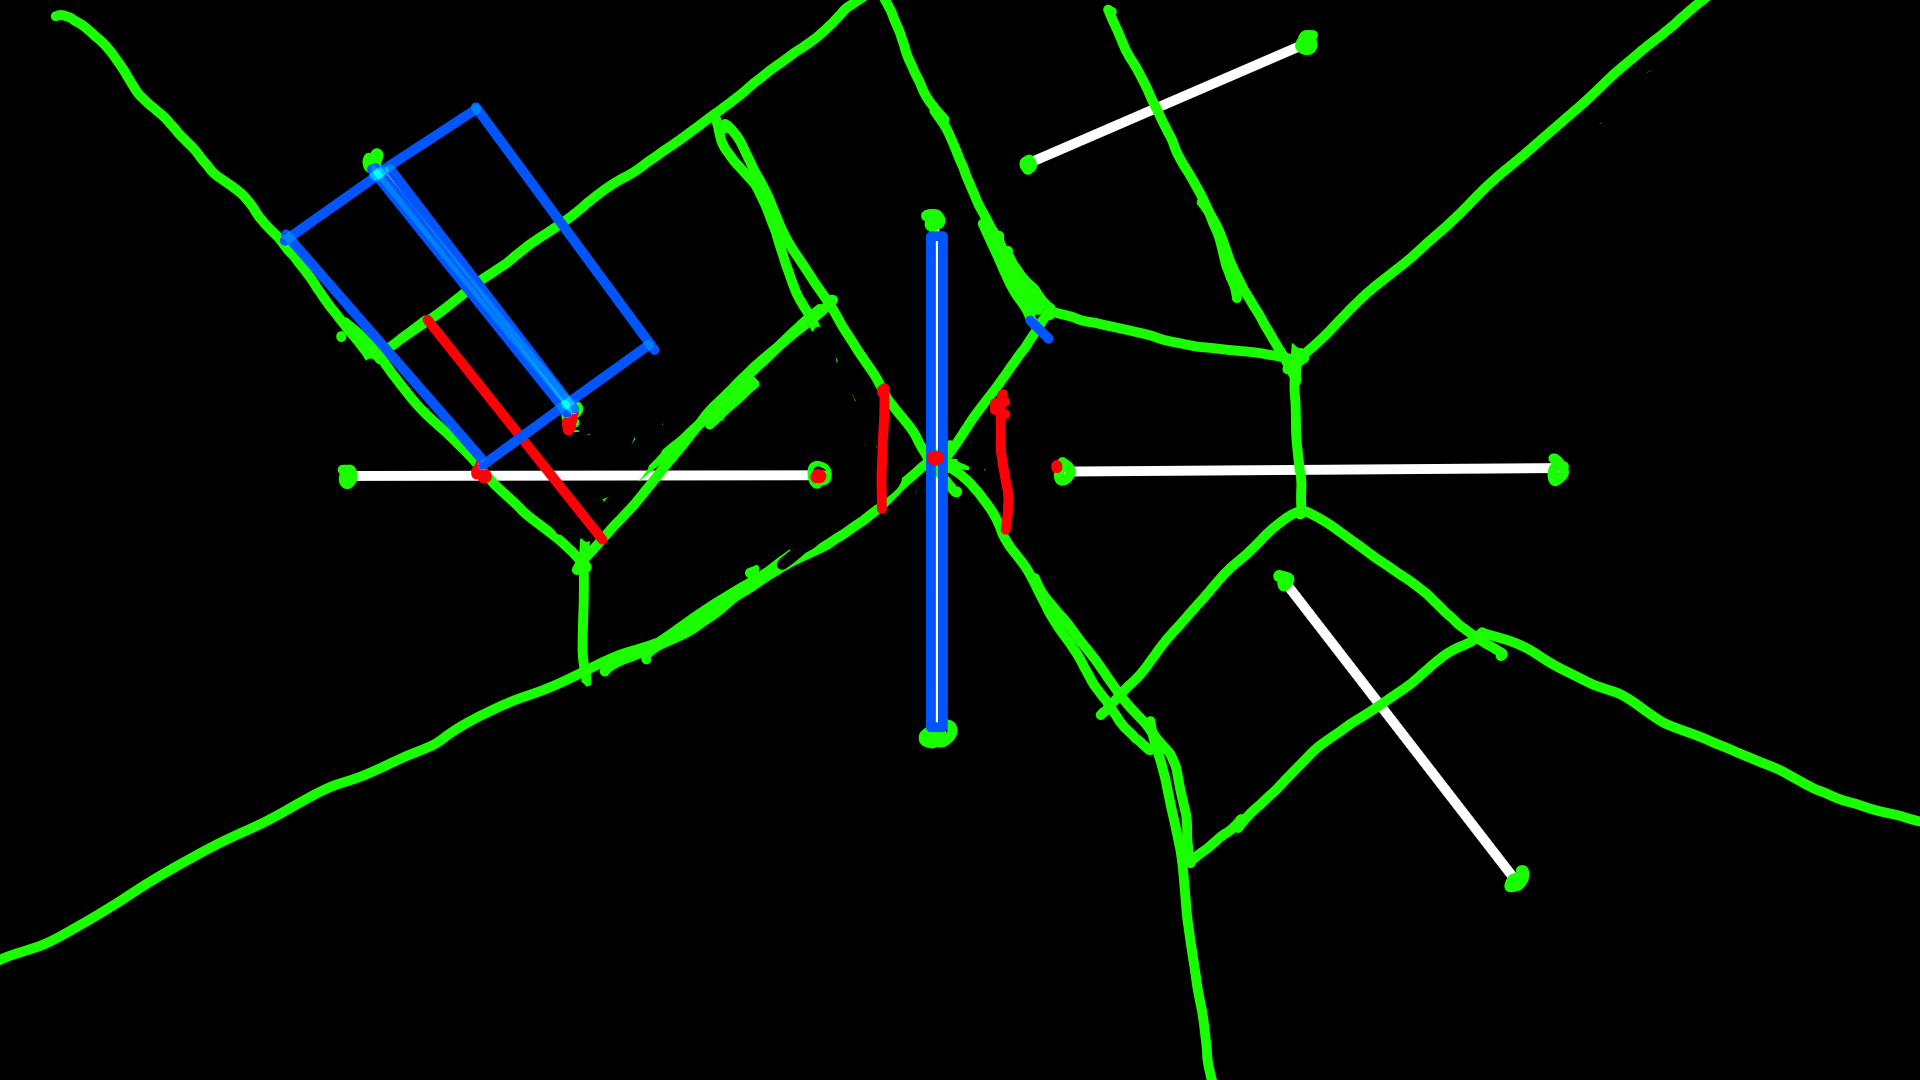
\includegraphics[width=\linewidth]{Step6.png}
		\caption{Widen rectangle until a conflict with another cell is found and repeat conflict voronoi calculation}
		\label{fig:Step6}
	\end{subfigure}
\end{figure}

\begin{figure}[h!]
	\centering
	\begin{subfigure}{0.3\linewidth}
		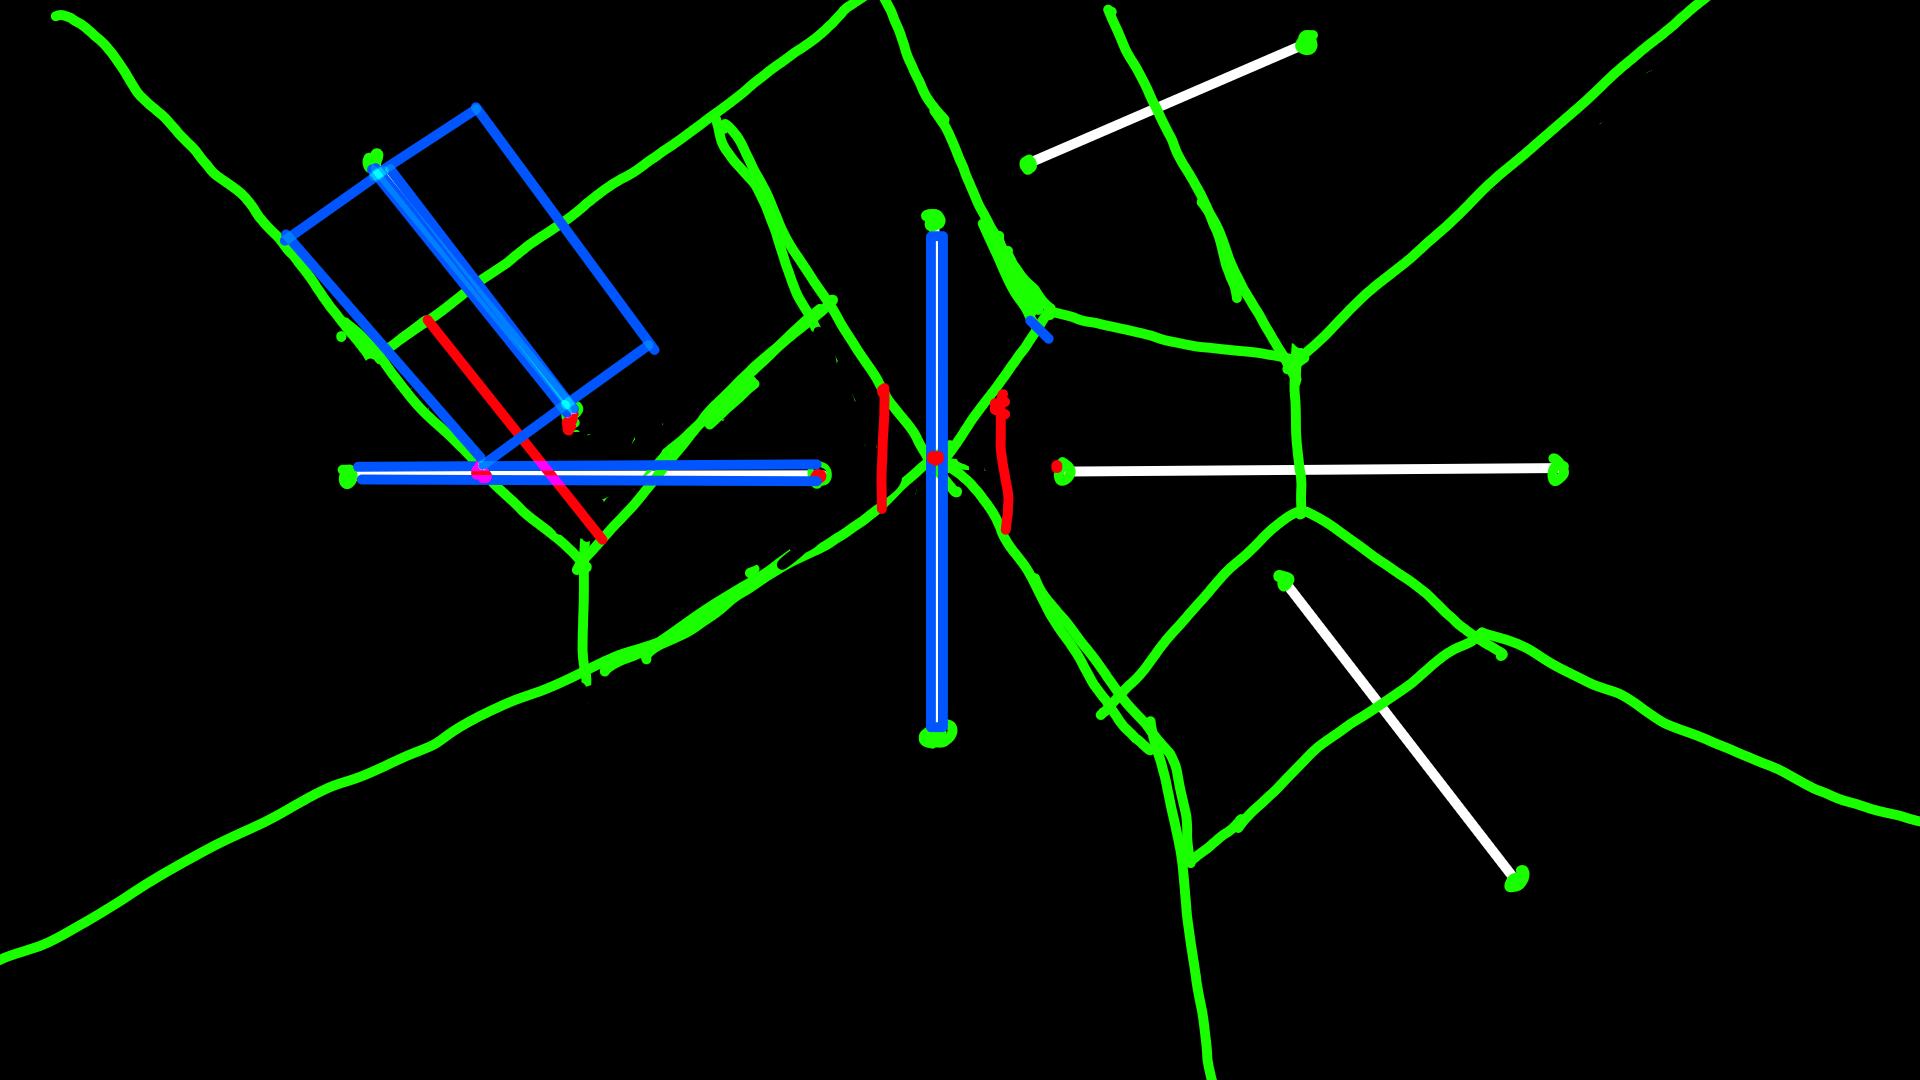
\includegraphics[width=\linewidth]{Step7.png}
		\caption{Repeat rectangle extension and conflict boundary calculation}
		\label{fig:Step7}
	\end{subfigure}%
	\hfill
	\begin{subfigure}{0.3\linewidth}
		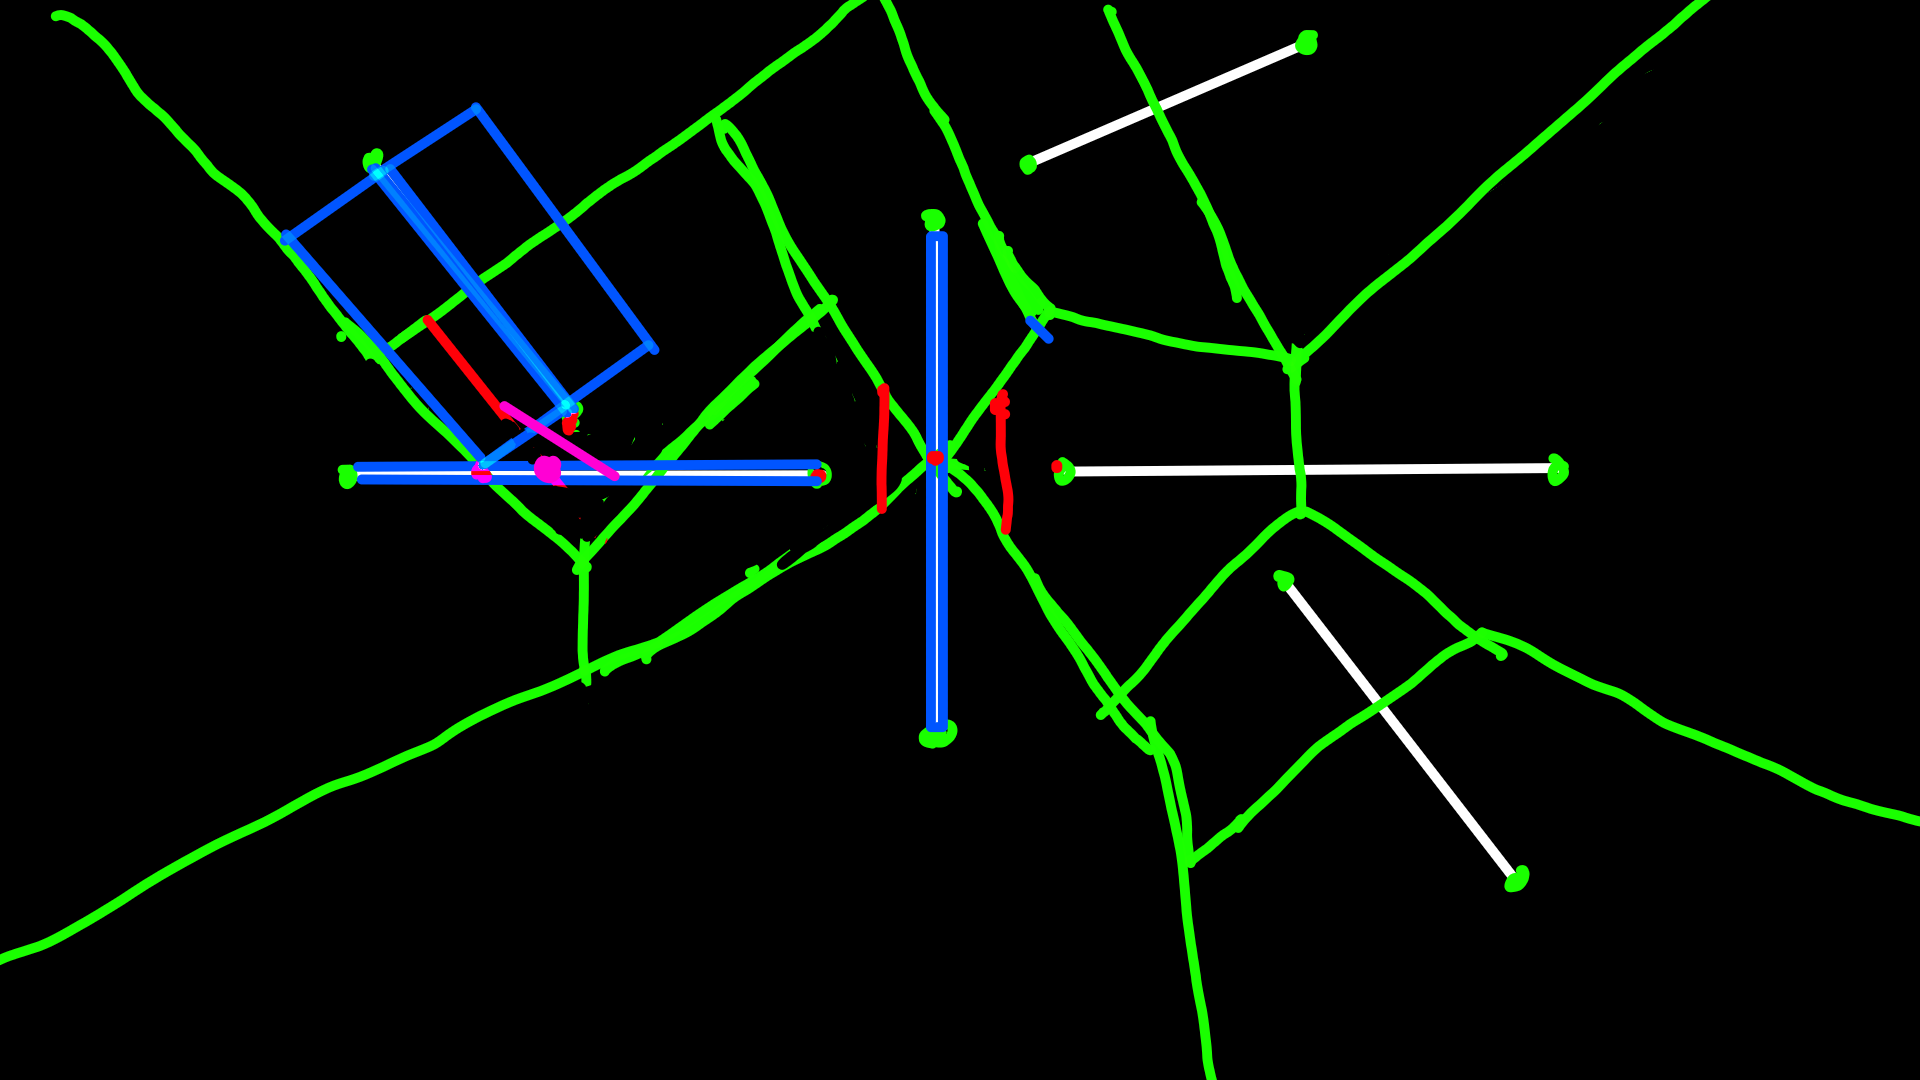
\includegraphics[width=\linewidth]{Step8.png}
		\caption{Adjust boundary of voronoi from previous step for intersection.}
		\label{fig:Step8}
	\end{subfigure}%
	\hfill
	\begin{subfigure}{0.3\linewidth}
		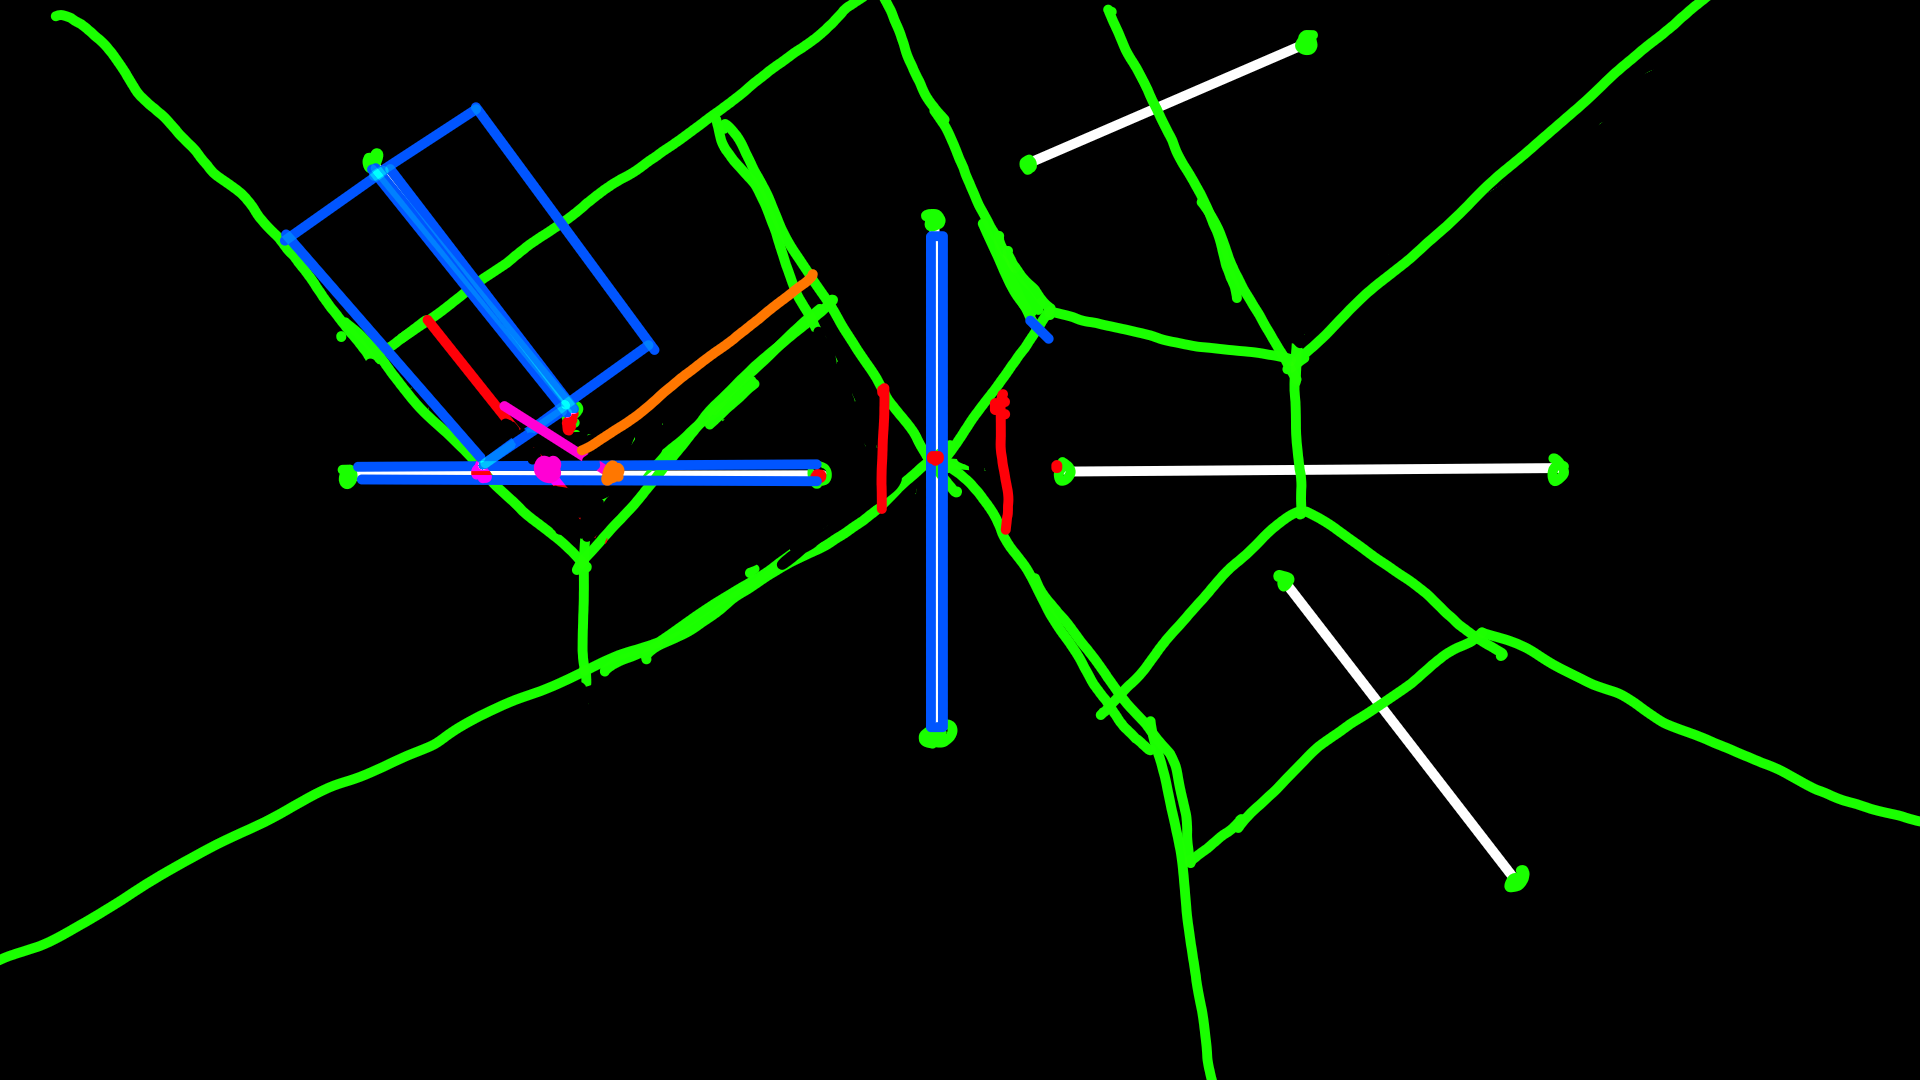
\includegraphics[width=\linewidth]{Step9.png}
		\caption{Calculate cell boundary for intersection with boundary from last step.}
		\label{fig:Step9}
	\end{subfigure}
\end{figure}

\section{Question 2}
The goal is to find the shortest path between two points for a disk of radius, r, given a 
set of points (assumedly obstacles), and the voronoi diagram of those points.
We construct a graph from the voronoi diagram where intersections between three or more voronoi cells are nodes,
and the intersections of two edges are edges. 
We then search through adjacent cells and remove pairings which have their defining points at a
distance of less than r from eachother. 
On the remaining edges we define their weights to be the euclidean distance they travel. 
We then check to ensure that at least one edge leads to the target point, and one
edge leads from the source point. 
If either check fails we report no solution and terminate.
Otherwise we run a shortest path algorithm such as Dijkstra's algorithm, and report
the result. 

\section{Question 3}

\end{document}

